\section{Simulation Results}
\label{sec:simulations}

\subsection{Simulation Settings}
\label{sec:simulation-settings}

\subsubsection{Channel Dataset and System Parameters}
The default system parameters are listed in
Table~\ref{tab:simulation-parameters}. Devices are uniformly distributed
within the satellite beam, and their delays, Doppler shifts, and array
responses follow the satellite-device geometry. Large-scale effects are
compensated. Channels follow the NTN-TDL-D profile \cite{shen2025},
with delay spread uniformly distributed over $[30,50]$~ns. The
line-of-sight gain has fixed amplitude and uniform phase, and the
diffuse gains are proper complex Gaussian.
We generate $50{,}000$ training channels and $5{,}000$ validation
channels of size $16\times16\times16$.

For $Q\leq KN$, the pilots are constructed from distinct DFT rows
$r_q\in\{0,\ldots,KN-1\}$, with a column permutation
$\{c_{kn}\}_{k,n}$ of the same set and independent phases
$\phi_{kn}\sim\mathcal U[0,2\pi)$:

\begin{equation}
 [\mathbf p_{qk}]_n=\sqrt{\frac{E_p}{N}}
 e^{-\mathrm j2\pi r_qc_{kn}/(KN)}e^{\mathrm j\phi_{kn}},
 \label{eq:pilot}
\end{equation}
with $\sum_{n=0}^{N-1}|[\mathbf p_{qk}]_n|^2=E_p$.

The received SNR is defined as the average signal power over the $QMN$
entries of $\mathbf A\mathbf X$ divided by $\sigma^2$. We set
$\sigma^2$ separately for each scene to obtain the specified SNR.

\begin{table}[!t]
\caption{Simulation Parameters}
\label{tab:simulation-parameters}
\centering
\small
\begin{tabular}{@{}ll@{}}
\toprule
Parameter & Value \\
\midrule
Carrier frequency $f_c$ & $2$~GHz \\
Satellite altitude & $600$~km \\
Beam radius & $128$~km \\
Minimum elevation angle & $30^\circ$ \\
UPA dimensions $M_y\times M_z$ & $4\times4$ \\
Array element spacing $d_y,d_z$ & $\lambda/2$ \\
Number of chirp subcarriers $N$ & $16$ \\
Subcarrier spacing $\Delta f$ & $30$~kHz \\
Chirp parameters $(c_1,c_2)$ & $(7/32,1/320)$ \\
CPP length $N_{\rm CPP}$ & $336$ \\
Differential-delay range & $[0,699]~\mu$s \\
Doppler-shift range & $[-41,41]$~kHz \\
Power delay profile & NTN-TDL-D \\
Delay spread & $[30,50]$~ns \\
Rician factor & $11.707$~dB \\
Default $(K,Q,p)$ & $(40,16,0.1)$ \\
\bottomrule
\end{tabular}
\end{table}

\subsubsection{Network Architectures and Training}
\label{sec:network-settings}
\label{sec:training-settings}
The denoiser uses the RefineNet \cite{lin2017} variant in
\cite{song2019}, with $2M$ real and imaginary input maps over
$N\times N$ DAFT coordinates.
Each stage contains two residual blocks, each with two
$3\times3$ convolutions, conditional instance normalization, and
exponential linear unit (ELU) activations.
The stage outputs are combined by four refinement blocks that restore
the spatial resolution, with $3\times3$ convolutions at the network
input and output. Table~\ref{tab:network-architectures} lists the channel
widths and spatial resolutions of both networks.

\begin{table}[!t]
\caption{Network Architectures}
\label{tab:network-architectures}
\centering
\small
\setlength{\tabcolsep}{3pt}
\begin{tabular}{@{}lcc@{}}
\toprule
Layer or stage & Channels & Map size \\
\midrule
\multicolumn{3}{@{}l}{\textit{Channel denoiser}} \\
Input convolution & $128$ & $N\times N$ \\
Residual stage 1 & $128$ & $N\times N$ \\
Residual stage 2 & $256$ & $N/2\times N/2$ \\
Residual stage 3 (dilation 2) & $256$ & $N/2\times N/2$ \\
Residual stage 4 (dilation 4) & $256$ & $N/2\times N/2$ \\
Refinement blocks 1--2 & $256,256$ & $N/2\times N/2$ \\
Refinement block 3 & $128$ & $N/2\times N/2$ \\
Refinement block 4 & $128$ & $N\times N$ \\
Output convolution & $2M$ & $N\times N$ \\
\midrule
\multicolumn{3}{@{}l}{\textit{Activity classifier}} \\
Convolutional stage 1 & $64$ & $N\times N$ \\
Convolutional stage 2 & $128$ & $N/2\times N/2$ \\
Convolutional stage 3 & $128$ & $N/4\times N/4$ \\
Fully connected layers & $128,1$ & --- \\
\bottomrule
\end{tabular}
\end{table}

Noise conditioning uses an embedding of $\log(v)/5$, formed by two
$64$-unit fully connected layers with sigmoid-weighted linear unit
(SiLU) activations and linearly projected to the normalization layers.
The denoiser also adopts the preconditioning in \cite{karras2022}:

\begin{equation}
 \begin{aligned}
 \mathbf f_\theta(\mathbf u,v)
 &=c_{\rm skip}(v)\mathbf u+c_{\rm out}(v)
   \mathbf g_\theta(c_{\rm in}(v)\mathbf u,v),\\
 c_{\rm in}(v)&=(\sigma_{\rm d}^2+v/2)^{-1/2},\\
 c_{\rm skip}(v)&=\frac{\sigma_{\rm d}^2}{\sigma_{\rm d}^2+v/2},\\
 c_{\rm out}(v)&=\left(\frac{\sigma_{\rm d}^2 v/2}
 {\sigma_{\rm d}^2+v/2}\right)^{1/2}.
 \end{aligned}
 \label{eq:mean-preconditioning}
\end{equation}

Here $\sigma_{\rm d}^2=1/2$ is the nominal variance per real coordinate after
normalization, and $\mathbf g_\theta$ is the RefineNet described above.

The classifier estimates the log likelihood ratio from $4M$ real and
imaginary maps of $\mathbf R$ and $\mathbf F_\theta(\mathbf R,v)$,
scaled by $\sqrt{2/(1+v)}$, together with five scalars:
$\log(v)/5$, logarithmic transforms of input/output/residual energies
normalized by $Dv$, and a sign-preserving logarithmic transform of the
real inner product normalized by $Dv$.
Its three convolutional stages each contain two $3\times3$ convolutions
with SiLU activations and padding $1$. Downsampling uses stride $2$ in
the first convolution of stages~2--3; the remaining convolutions use
stride $1$.
Noise conditioning is provided by a $64$-unit fully connected SiLU
embedding of $\log(v)/5$, whose linear projections are added to the
stage outputs. The flattened features and five scalars are combined by
the fully connected layers in Table~\ref{tab:network-architectures},
with SiLU between them, to produce one logit per device.

We train the denoiser by minimizing \eqref{eq:first-loss} with the
preconditioning in \eqref{eq:mean-preconditioning}. The variance $v$
is sampled uniformly on a logarithmic scale over $[10^{-3},10^2]$.
We use Adam for $200$ epochs with batch size $64$, initial learning
rate $10^{-4}$, and exponential moving average decay $0.999$.
STMP uses the same clean channels and number of epochs.

With the denoiser fixed, we train the classifier using
\eqref{eq:classifier-loss} for $100$ epochs, with batch size $32$
and initial learning rate $3\times10^{-4}$. For both networks, we select
the model with the lowest validation loss.

\subsubsection{Compared Receivers}
\label{sec:compared-receivers}
We compare GP-MP with five baselines. GP-MP-EP uses estimated phases;
the other configurations use known phases:
\begin{itemize}[leftmargin=*,topsep=2pt,itemsep=2pt,parsep=0pt]

\item \textbf{STMP:} We adapt STMP \cite{cai2026} to the multi-frame
AFDM model, retaining its white-noise-trained first- and second-order
score networks for conditional mean and variance estimation. We replace
its Gaussian-message-based activity-probability update with a learned
density-ratio estimator trained using the corresponding first-order network.
\begin{samepage}
\item \textbf{Simultaneous orthogonal matching pursuit (SOMP)}
\cite{TroppGilbertStrauss2006SOMP}: This method selects dictionary atoms
shared by the receive antennas and estimates their coefficients by
least squares. We use an integer delay--Doppler dictionary
and select up to $64$ atoms.
\par
\end{samepage}
\item \textbf{GAMP-SBL:} This method uses generalized approximate message
passing in sparse Bayesian learning \cite{ZhangFanHaoQuan2023GAMPSBL}.
Our implementation uses the integer delay--Doppler dictionary,
shares row precisions across receive antennas, and allows up to
$1{,}000$ iterations.
\item \textbf{GNN-ASPL:} This method alternates AMP-based channel estimation
with adaptive sparsity pattern learning using a graph neural network
\cite{ding2026}. It uses the same integer delay--Doppler dictionary and
a $10$-layer network.
\item \textbf{Off-grid SBL:} In addition to the channel coefficients,
this method estimates continuous delay and Doppler offsets through a
first-order linear approximation of the dictionary
\cite{WeiEtAl2022OffgridSBL}. We allow up to $120$ iterations.
For the SNR comparison, the $7$, $13$, and $25$ Doppler grid points
are paired with $12$, $24$, and $48$ retained candidates per device
and $48$, $96$, and $192$ offset candidates per iteration, respectively;
all three configurations use $112$ delay grid points.
\end{itemize}

\subsubsection{Evaluation Settings and Metrics}
\label{sec:receiver-settings}
\label{sec:stopping-criteria}
Phase estimation in GP-MP-EP covers $d\in[0,N)$ and
$|\nu|\leq\nu_{\max}$, where $\nu_{\max}$ is the channel model's Doppler
bound. Pilot correlations over $128$ phase bins identify three coarse
candidates. The Doppler values corresponding to each candidate phase
within this bound form the initial search set, from which the best
$12$ are refined by at most $25$ L-BFGS-B iterations per candidate.

All receivers estimate the noise variance from the observations.
STMP and GP-MP use an activity threshold of $0.5$ and default damping factors
of $0.2$ and $0.4$, respectively.
Their iterations are bounded by $I_{\min}=60$ and $I_{\max}=600$,
with a relative-change tolerance of $5\times10^{-4}$.
After $I_{\min}$ iterations, convergence is assessed from the stability
of channel and activity estimates and the consistency of variance
updates.
\ifdefined\FullManuscript
The complete stopping checks and tolerances are given in
Appendix~\ref{app:implementation-settings}.
\fi

GP-MP uses $L_z=1$ and $\delta_{\rm FD}=10^{-2}$ in
\eqref{eq:derivative-trace}. The average conditional variance has a
lower bound $\tau_{\min}=10^{-4}$.

The evaluation protocol specifies $1{,}000$ Monte Carlo trials per
operating point.
\ifdefined\FullManuscript
Appendix~\ref{app:evaluation-protocol} gives the evaluation protocol.
\fi

For scenes $e\in\mathcal T$, the normalized mean-squared error (NMSE)
is the total squared Frobenius error between
$\widehat{\mathbf X}_{ek}$ and $\mathbf X_{ek}$ divided by the total
squared Frobenius norm of $\mathbf X_{ek}$. Both totals include all
scenes in $\mathcal T$ and all $K$ devices;
the ratio is expressed in decibels. For channel denoising, the same
metric uses $\mathbf H$ in place of $\mathbf X$ and is accumulated
over individual channel samples. The activity error rate (AER) is the
total number of missed detections and false alarms divided by
$K|\mathcal T|$.

\begin{figure}[!t]
\centering
\makebox[\columnwidth][c]{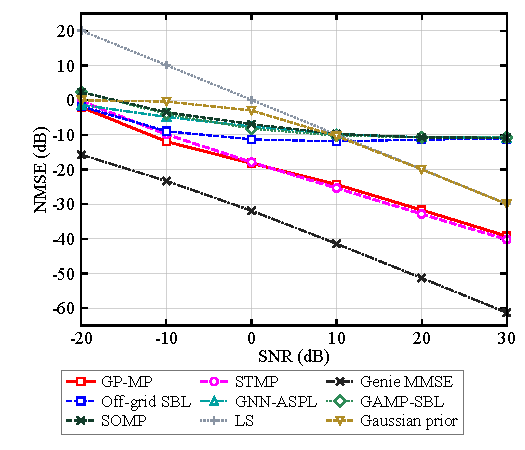
\includegraphics[width=88.9mm]{channel_denoising.pdf}}
\caption{Channel denoising under AWGN with known variance.}
\label{fig:cstmp-denoising}
\end{figure}

\begin{table}[!t]
\caption{Activity Detection Performance and Iteration-Limit Rates}
\label{tab:activity-evidence}
\centering
\small
\setlength{\tabcolsep}{2pt}
\begin{tabular}{@{}rcccccccc@{}}
\toprule
& \multicolumn{4}{c}{STMP}
& \multicolumn{4}{c}{GP-MP} \\
\cmidrule(lr){2-5}\cmidrule(l){6-9}
& \multicolumn{2}{c}{Gaussian} & \multicolumn{2}{c}{Density ratio}
& \multicolumn{2}{c}{Gaussian} & \multicolumn{2}{c}{Density ratio} \\
\cmidrule(lr){2-3}\cmidrule(lr){4-5}\cmidrule(lr){6-7}\cmidrule(l){8-9}
\shortstack{SNR\\(dB)} & \shortstack{AER\\(\%)} & \shortstack{Limit\\(\%)}
& \shortstack{AER\\(\%)} & \shortstack{Limit\\(\%)}
& \shortstack{AER\\(\%)} & \shortstack{Limit\\(\%)}
& \shortstack{AER\\(\%)} & \shortstack{Limit\\(\%)} \\
\midrule
$-4$ & $9.225$ & $2$ & $0.525$ & $0$ & $44.575$ & $63$ & $0.200$ & $0$ \\
$-2$ & $7.875$ & $3$ & $0.225$ & $0$ & $43.475$ & $55$ & $0.125$ & $0$ \\
$0$ & $6.375$ & $2$ & $0.100$ & $0$ & $40.975$ & $46$ & $0.075$ & $0$ \\
$2$ & $5.550$ & $1$ & $0.050$ & $0$ & $36.750$ & $31$ & $0.025$ & $0$ \\
$4$ & $4.800$ & $1$ & $0.025$ & $0$ & $32.050$ & $19$ & $0.025$ & $0$ \\
$6$ & $4.225$ & $0$ & $0.025$ & $0$ & $27.425$ & $11$ & $0.025$ & $0$ \\
\bottomrule
\end{tabular}
\end{table}

\begin{figure}[!t]
\centering
\makebox[\columnwidth][c]{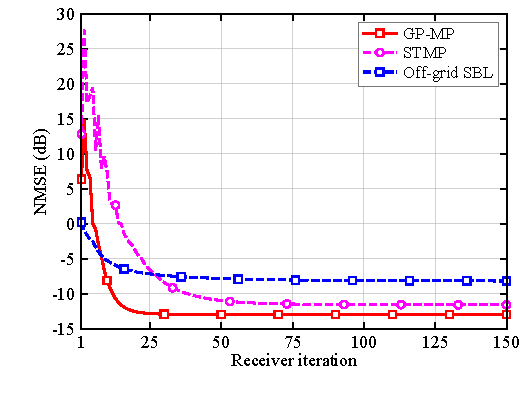
\includegraphics[width=88.9mm]{convergence.pdf}}
\caption{NMSE versus iteration at $0$~dB, with $K=40$, $Q=16$,
and $p=0.1$.}
\label{fig:cstmp-convergence}
\end{figure}

\begin{figure}[!t]
\centering
\makebox[\columnwidth][c]{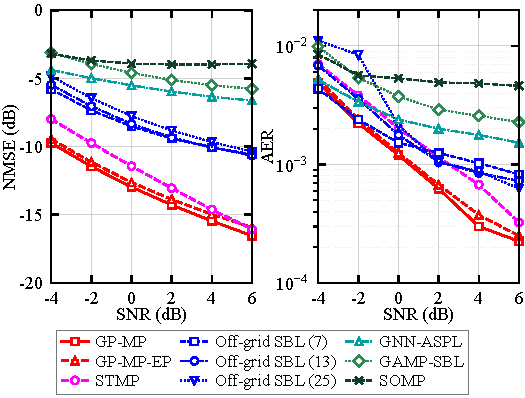
\includegraphics[width=88.9mm]{snr_comparison.pdf}}
\caption{Channel NMSE and AER versus SNR with $K=40$, $Q=16$,
and $p=0.1$.}
\label{fig:cstmp-snr}
\end{figure}

\begin{figure}[!t]
\centering
\makebox[\columnwidth][c]{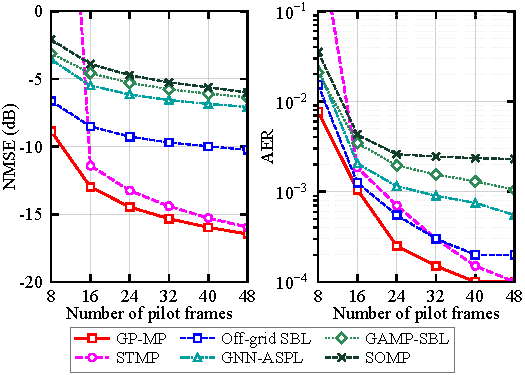
\includegraphics[width=88.9mm]{pilot_frames.pdf}}
\caption{Channel NMSE versus the number of pilot frames at
$0$~dB, with $K=40$ and $p=0.1$.}
\label{fig:cstmp-pilots}
\end{figure}

\begin{figure}[!t]
\centering
\makebox[\columnwidth][c]{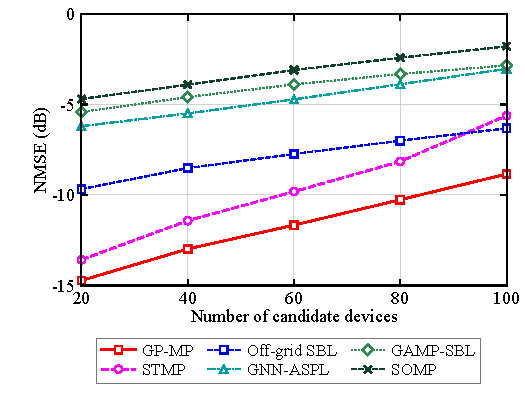
\includegraphics[width=88.9mm]{user_count.pdf}}
\caption{Channel NMSE versus the number of candidate devices
at $0$~dB, with $Q=16$ and $p=0.1$.}
\label{fig:cstmp-users}
\end{figure}

\begin{figure}[!t]
\centering
\makebox[\columnwidth][c]{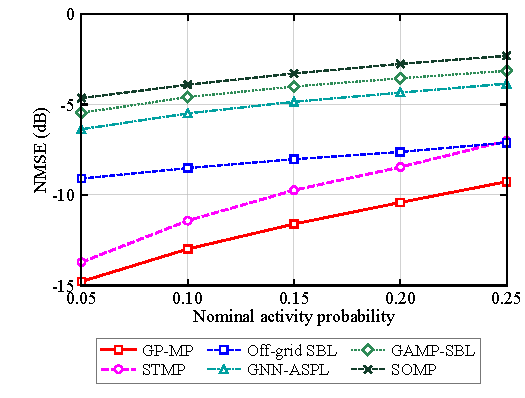
\includegraphics[width=88.9mm]{activity_probability.pdf}}
\caption{Channel NMSE versus nominal activity probability at
$0$~dB, with $K=40$ and $Q=16$.}
\label{fig:cstmp-activity}
\end{figure}

\begin{figure*}[!t]
\centering
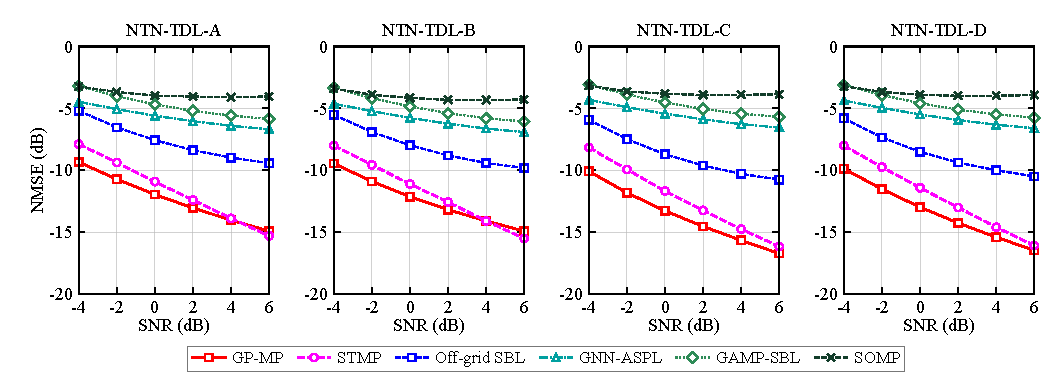
\includegraphics[width=177.8mm]{cross_channel.pdf}
\caption{Channel NMSE for NTN-TDL profiles A, B, C, and D (from left
to right), with $K=40$, $Q=16$, and $p=0.1$.}
\label{fig:cstmp-cross}
\end{figure*}

\subsection{Channel Denoising Performance}
\label{sec:denoising-performance}
We first evaluate the channel denoisers under
$\mathbf R=\mathbf H+\mathbf W$, where
$\vect(\mathbf W)\sim\CN(\mathbf0,v\I)$ and $v$ is known.
The nominal SNR is $-10\log_{10}v$ and takes six values from
$-20$ to $30$~dB. The reference estimators are:
\begin{itemize}[leftmargin=*,topsep=2pt,itemsep=2pt,parsep=0pt]
\item \textbf{Least squares (LS):} The estimate is the noisy observation
$\mathbf R$.
\item \textbf{Gaussian-prior estimate:} The estimate is
$\widehat P_H\mathbf R/(\widehat P_H+v)$, where $\widehat P_H$ is the
training-channel power.
\item \textbf{Genie-aided conditional MMSE:} We compute the analytic
conditional MSE of the remaining Gaussian gains given the true path
geometry, powers, and line-of-sight gain.
\end{itemize}
We also evaluate the four sparse-recovery baselines in this denoising
setting.

Figure~\ref{fig:cstmp-denoising} shows that both learned denoisers
achieve lower NMSE than LS and the Gaussian-prior estimate throughout
the tested SNR range. Their advantage over the sparse-recovery baselines
increases at moderate and high SNR, where these baselines approach error
floors while the NMSE of the learned denoisers continues to decrease.
The GP-MP denoiser yields lower NMSE at low SNR, whereas the STMP
denoiser yields lower NMSE at high SNR.
Both remain above the genie-aided reference.

\subsection{Effect of Density Ratio Estimation}
\label{sec:activity-evidence}
To assess density ratio estimation, we compare the learned activity
update with the Gaussian approximation

\begin{align}
 \ell_k^{\rm G}&=\frac{\norm{\mathbf R_k}_F^2}{v}
 -\frac{\norm{\mathbf R_k-\mathbf E_k}_F^2}{\tau_k^{\rm ext}+v}
 \notag\\
 &\quad-D\log\left(1+\frac{\tau_k^{\rm ext}}{v}\right),
 \label{eq:gaussian-evidence}\\
 p_k&=\sigmoid(\logit\rho+\ell_k^{\rm G}).
 \label{eq:gaussian-activity}
\end{align}

For both STMP and GP-MP, we change only the activity update and keep
the remaining settings fixed. Table~\ref{tab:activity-evidence} reports
the AER over
all runs and the percentage reaching the $600$-iteration limit (Limit).

Table~\ref{tab:activity-evidence} shows that, for both receivers, the
learned activity update yields lower AER than the Gaussian update at
every tested SNR. No run using the learned update reaches the iteration
limit, whereas some runs using the Gaussian update do. The improvement
is larger for GP-MP, although STMP performs better
under the Gaussian update. These results support the effectiveness of
density ratio estimation for activity detection under the learned
channel prior.

\subsection{JADCE Performance}
\label{sec:jadce-performance}
Unless stated otherwise, the default parameters in
Table~\ref{tab:simulation-parameters} are used.

Figure~\ref{fig:cstmp-convergence} compares the NMSE trajectories with
early stopping disabled. The GP-MP curve
stabilizes earlier and at a lower NMSE than STMP. Off-grid SBL also
levels off, but with a larger estimation error. GP-MP therefore achieves
a more accurate channel estimate within fewer iterations than STMP.

Figure~\ref{fig:cstmp-snr} compares channel NMSE and AER over SNRs
from $-4$ to $6$~dB. GP-MP achieves the lowest NMSE throughout this
range, with an approximately $1.5$~dB advantage over STMP at $0$~dB.
Its advantage over STMP decreases as SNR increases, whereas the gap
to the sparse-recovery baselines widens. Off-grid SBL is the most
accurate of the four sparse-recovery baselines, and GP-MP outperforms
all three Off-grid SBL configurations.

The AER also generally decreases with SNR. GP-MP has lower AER than
STMP throughout this SNR range and outperforms the four sparse-recovery
baselines at moderate and high SNR. These results demonstrate improved
JADCE performance with a denoiser that provides channel estimates and
average variance without a separately trained variance model.

With estimated phases, GP-MP-EP incurs an NMSE increase of
$0.28$--$0.60$~dB relative to GP-MP, while its AER remains close to
the known-phase result. This comparison shows that estimating the
phases from pilot observations retains most of the known-phase
receiver's performance over this SNR range.

Figure~\ref{fig:cstmp-pilots} shows channel NMSE as $Q$ increases from
$8$ to $24$. With fixed energy per frame, additional frames provide more
observations and generally reduce NMSE. GP-MP and GP-MP-EP achieve
lower NMSE than all baselines at each frame count. For an NMSE target
of $-12$~dB, both reach the target at $16$ frames, compared with $20$
frames for STMP, corresponding to a $20\%$ reduction in pilot frames.

STMP exhibits severe degradation at low pilot counts: its NMSE is
$34.70$~dB at $Q=8$ and $-4.78$~dB at $Q=12$, compared with
$-8.88$~dB and $-11.61$~dB for GP-MP, respectively. This pronounced
loss indicates that STMP is more sensitive to limited pilot observations.
GP-MP-EP incurs an NMSE increase of $0.30$--$0.41$~dB relative to
GP-MP across these frame counts.

Figure~\ref{fig:cstmp-users} compares NMSE as the number of candidate
devices increases from $K=20$ to $100$. With the activity probability
and pilot-frame count fixed, both the number of candidate channels and
the expected number of active devices increase. The NMSE therefore
increases for all methods. GP-MP
maintains the lowest NMSE, with a growing advantage over STMP as $K$
increases. This demonstrates its effectiveness at higher device loads
with the available pilot and antenna resources.

Figure~\ref{fig:cstmp-activity} shows NMSE for nominal activity
probabilities from $0.05$ to $0.25$. Increasing the activity probability
increases the expected number of active devices, while the numbers of
candidate devices, pilot frames, and receive antennas remain fixed.
The NMSE increases for all methods. GP-MP maintains the lowest NMSE,
with a smaller increase than STMP. Its larger advantage at higher
activity probabilities indicates
better tolerance to increasing activity loads.

\subsection{Comparison Across Channel Profiles}
To examine performance under channel mismatch, we apply the networks
trained on NTN-TDL-D to profiles A, B, and C without retraining.

Figure~\ref{fig:cstmp-cross} shows that GP-MP outperforms the four
sparse-recovery baselines on all four profiles. This indicates that the
learned prior remains effective across these channel profiles. The relative
performance of the two learned receivers depends on the profile and
SNR; STMP is more accurate on profiles A and B at $6$~dB.
